\documentclass[usenames,dvipsnames]{beamer}
\usetheme{Berlin}
\usepackage[utf8]{inputenc}
\usepackage[english]{babel}
\usepackage{graphicx}
\usepackage{url}
\usepackage{multicol}
\usepackage{relsize}
\usepackage{fancyvrb}

\graphicspath{ {images/} }

\title{Seccomp - another kernel security mechanism}
\subtitle{}
\author{Alexander Livenets \\ Peter Poljak}
\institute{}
\date{20 July 2020}

\newcommand{\codeinline}[1] {\texttt{\smaller[2]{#1}}}
\newcommand{\greenalert}[1] {\alert{\textcolor{green}{#1}}}
\newcommand{\redalert}[1] {\alert{\textcolor{red}{#1}}}
\begin{document}

\AtBeginSection[]
{
\begin{frame}
\frametitle{Table of Contents}
\tableofcontents[currentsection]
\end{frame}
}

\setbeamertemplate{endpage}{%
\begin{frame}
\center \Huge Thanks!
\end{frame}
}

\begin{frame}
\titlepage
\end{frame}

\section{Tutorial}
\subsection{Kernel syscalls}
\begin{frame}
\frametitle{\subsecname}
\centering
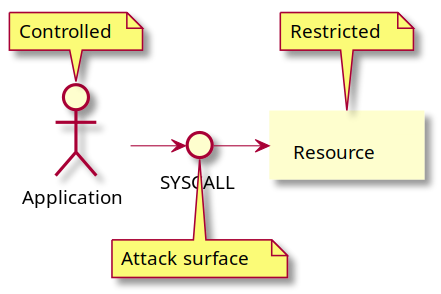
\includegraphics[scale=0.5]{images/surface-001.png}
\end{frame}

\begin{frame}
\frametitle{\subsecname}
\centering
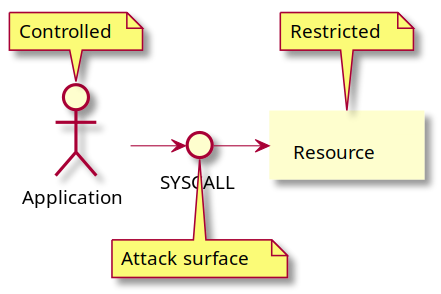
\includegraphics[scale=0.5]{images/surface-001.png}
\end{frame}

\subsection{What is seccomp?}
\begin{frame}
\frametitle{\subsecname}
\begin{itemize}
\item seccomp == SECure COMPuting
\item Kernel provides large number of system calls (\textbf{\~400} system calls)
\item Each system call is a vector for attack against kernel
\item Most programs use only small subset of available system calls
\item Remaining systems calls should never occur
\item If they do occur, perhaps it is because program has been compromised
\item \textbf{Seccomp} = mechanism to restrict the system calls that a process may make
  \begin{itemize}
  \item{Reduces attack surface of kernel}
  \item{A key component for building application sandboxes}
  \end{itemize}
\end{itemize}
\end{frame}

\subsection{seccomp filtering}
\begin{frame}
\frametitle{Strict seccomp mode}
\begin{itemize}
  \item 
  \begin{itemize}
    \item only permitted system calls are read(), write(), \_exit(), and sigreturn() 
    \item Note: open() not included (must open files before entering strict mode)
    \item sigreturn() allows for signal handlers
    \item Other system calls $\rightarrow$ SIGKILL
  \end{itemize}
\end{itemize}
\end{frame}

\begin{frame}
\frametitle{Filter mode}
\begin{itemize}
\item Seccomp filters are expressed as BPF (Berkeley Packet Filter) programs
\item BPF originally devised (in 1992) for tcpdump and network packet filtering
\item BPF allows in-kernel selection of packets. Filtering is based on fields in packet header
\item Filtering in kernel more efficient than filtering in user space
  \begin{itemize}
    \item Unwanted packet are discarded early
    \item Avoid passing every packet over kernel-user-space boundary
  \end{itemize}
\end{itemize}
\end{frame}

\subsection{BPF}
\begin{frame}
\frametitle{\subsecname}
BPF defines a virtual machine (VM) that can be implemented inside kernel
\begin{itemize}
  \item Simple instruction set
  \item All instructions are same size (64 bits)
  \item Implementation is simple and fast
  \item Only branch-forward instructions. Programs are directed acyclic graphs (DAGs)
  \item Easy to verify validity/safety of BPF programs
  \item Program completion is guaranteed (DAGs)
  \item Simple instruction set ⇒ can verify opcodes and arguments
  \item Can detect dead code
  \item Can verify that program completes via a “return” instruction
  \item BPF filter programs are limited to 4096 instructions
\end{itemize}
\end{frame}

\section{seccomp programming}
\begin{frame}[fragile]
\frametitle{\secname}
Seccomp provides data describing syscall to filter program
Buffer is read-only
I.e., seccomp filter can’t change syscall or syscall arguments
Can be expressed as a C structure...
\begin{verbatim}
struct seccomp_data {
  int nr; /* System call number */
  __u32 arch; /* AUDIT_ARCH_ * value */
  __u64 instruction_pointer; /* CPU IP */
  __u64 args[6]; /* System call arguments */
};
\end{verbatim}
\end{frame}

\subsection{seccomp features}
\begin{frame}
\frametitle{\subsecname}
\begin{itemize}
\item Once a filter is installed, each system call is tested against filter
\item Seccomp filter MUST return a value to kernel indicating whether system call is permitted. Otherwise EINVAL when attempting to install filter
\item Return value is 32 bits, in two parts:
\begin{itemize}
\item Most significant 16 bits (\codeinline{SECCOMP\_RET\_ACTION\_FULL} mask) specify an action to kernel
\item Least significant 16 bits (\codeinline{SECCOMP\_RET\_DATA} mask) specify “data” for return value
\end{itemize}
\end{itemize}
\end{frame}

\begin{frame}
\begin{itemize}
\item if existing filters permit prctl() or seccomp(), further filters can be installed
\item 32k maximum for total instructions in all filters
\item All filters are always executed, in reverse order of registration (LIFO style)
\item Each filter yields a return value
\item If seccomp filters permit fork() or clone(), then child inherits parent’s filters
\item If seccomp filters permit execve(), then filters are preserved across execve()
\end{itemize}
\end{frame}

\begin{frame}
Various possible filter return actions, including:
\begin{itemize}
\item \codeinline{SECCOMP\_RET\_ALLOW}: system call is allowed to execute
\item \codeinline{SECCOMP\_RET\_KILL\_PROCESS}: process (all threads) is killed. Terminated as though process had been killed with SIGSYS
\item \codeinline{SECCOMP\_RET\_KILL\_THREAD}: calling thread is killed/terminated as though thread had been killed with SIGSYS
\item \codeinline{SECCOMP\_RET\_ERRNO}: return an error from system call. System call is not executed
\item \codeinline{SECCOMP\_RET\_TRACE}, \codeinline{SECCOMP\_RET\_TRAP}, \codeinline{SECCOMP\_RET\_LOG}
\end{itemize}
\end{frame}

\begin{frame}[fragile]
\footnotesize
\begin{verbatim}
static void install_filter(void) {
struct sock_filter filter[] = {
  BPF_STMT(BPF_LD | BPF_W | BPF_ABS, 
      offsetof(struct seccomp_data, arch)),
  BPF_JUMP(BPF_JMP | BPF_JEQ | BPF_K, AUDIT_ARCH_X86_64, 1, 0),
  BPF_STMT(BPF_RET | BPF_K, SECCOMP_RET_KILL_PROCESS),
  BPF_STMT(BPF_LD | BPF_W | BPF_ABS,
      offsetof(struct seccomp_data , nr)),
  BPF_JUMP(BPF_JMP | BPF_JEQ | BPF_K, __NR_open, 2, 0),
  BPF_JUMP(BPF_JMP | BPF_JEQ | BPF_K, __NR_openat, 1, 0),
  BPF_STMT(BPF_RET | BPF_K, SECCOMP_RET_ALLOW),
  BPF_STMT(BPF_RET | BPF_K, SECCOMP_RET_KILL_PROCESS),
};
\end{verbatim}
\begin{itemize}
\item Load system call number into accumulator
\item Test if system call number matches \codeinline{\_\_NR\_open}
  \begin{itemize}
  \item True: advance two instructions $\rightarrow$ kill process
  \item False: advance 0 instructions $\rightarrow$ next test
  \end{itemize}
\item Test if system call number matches \codeinline{\_\_NR\_openat}
  \begin{itemize}
  \item True: advance one instruction $\rightarrow$ kill process
  \item False: advance 0 instructions $\rightarrow$ allow syscall
  \end{itemize}
\end{itemize}
\end{frame}

\begin{frame}[fragile]
\small
\begin{verbatim}
struct sock_fprog prog = {
  .len = (unsigned short)(sizeof(filter) / sizeof(filter[0])),
  . filter = filter,
};

seccomp(SECCOMP_SET_MODE_FILTER, 0, &prog);
\end{verbatim}
\end{frame}

\section{seccomp tools}
\begin{frame}
\begin{itemize}
  \item libseccomp (\url{https://github.com/seccomp/libseccomp})
  \item sandboxify (\url{https://github.com/cloudflare/sandbox})
\end{itemize}
\end{frame}

\subsection{libseccomp}
\begin{frame}[fragile]
\small
\begin{verbatim}
  scmp_filter_ctx ctx;
  ctx = seccomp_init(SCMP_ACT_ALLOW);
  seccomp_rule_add(ctx, SCMP_ACT_ERRNO(EPERM), SCMP_SYS(clone), 0);
  seccomp_rule_add(ctx, SCMP_ACT_ERRNO(ENOTSUP), SCMP_SYS(fork), 0);
  seccomp_load(ctx);
  if(fork() != -1)
    fprintf(stderr, "fork() succeeded\n");
  else
    perror ("fork");
\end{verbatim}
\end{frame}

\section{SystemD and seccomp}
\begin{frame}[fragile]
\frametitle{\secname}
\begin{verbatim}
[Service]
SystemCallFilter=open openat close socket recv
    recvfrom send sendto prctl execve
\end{verbatim}

\begin{verbatim}
[Service]
SystemCallFilter=@system-service
SystemCallErrorNumber=EPERM
\end{verbatim}
List of syscalls can be collected via usage of \codeinline{perf}/\codeinline{strace}
\end{frame}

\begin{frame}[fragile]
\frametitle{sandboxify}
\begin{verbatim}
SECCOMP_SYSCALL_ALLOW=exit_group:fstat:uname:write \
SECCOMP_SYSCALL_DENY=execve \
  sandboxify my-binaty
\end{verbatim}
\end{frame}

\begin{frame}[fragile]
\frametitle{Performance cost}
\centering
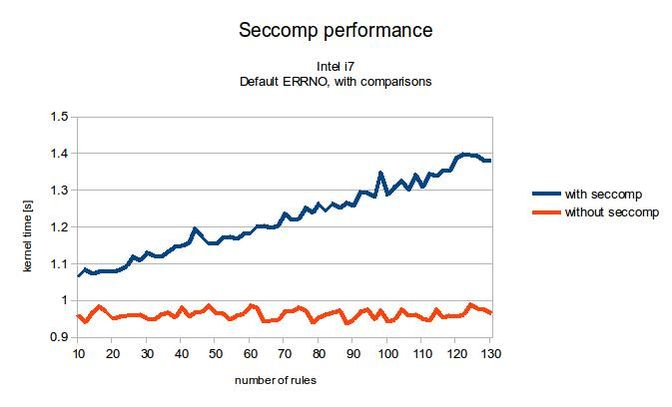
\includegraphics[scale=0.3]{images/672px-Seccomp_i7_extended_errno.jpg}

\raggedright

Factors that may affect the performance
  \begin{itemize}
    \item Order of filtering rules
    \item Structure of rules (return errno/kill process)
  \end{itemize}
\end{frame}

\begin{frame}
\frametitle{Caveats}
\begin{itemize}
\item Adding a seccomp filter can cause bugs in application
\item Filtering is based on syscall numbers, but applications normally call C library wrappers (not direct syscalls), which depend on the implementation and the version of C library
\end{itemize}
\end{frame}

\section{References}
\begin{frame}
\frametitle{\secname}
\footnotesize
\begin{itemize}
	\item \url{https://events19.linuxfoundation.org/wp-content/uploads/2017/12/Using-Seccomp-to-Limit-the-Kernel-Attack-Surface-Michael-Kerrisk-man7.org-Training-and-Consulting.pdf}
  \item https://prefetch.net/blog/2017/11/27/securing-systemd-services-with-seccomp-profiles/
  \item \codeinline{man 2 seccomp}
  \item \url{https://blog.cloudflare.com/sandboxing-in-linux-with-zero-lines-of-code/}
  \item \url{https://wiki.tizen.org/Security:Seccomp}
\end{itemize}
\end{frame}

\usebeamertemplate{endpage}

\end{document}
